\documentclass[12pt]{article}
\usepackage[margin=1in]{geometry}
\usepackage{graphicx}
\graphicspath{{../outputs/}}
\usepackage{booktabs}
\usepackage[dvipsnames,table]{xcolor}
\usepackage{hyperref}
\usepackage{amsmath}
\usepackage{float}
\usepackage{caption}
\usepackage{enumitem}
\usepackage{setspace}
\usepackage{parskip}
\usepackage{titlesec}
\usepackage[scaled]{helvet}
\renewcommand{\familydefault}{\sfdefault}
\onehalfspacing

% ── CareerDrive color palette ──────────────────────────────
\definecolor{cdprimary}{HTML}{8B4049}    % Burgundy
\definecolor{cdsecondary}{HTML}{C4918A}  % Rose
\definecolor{cdtertiary}{HTML}{E8C8C3}   % Light rose
\definecolor{cddark}{HTML}{4A2028}       % Dark burgundy
\definecolor{cdsurface}{HTML}{FDF5F3}    % Warm off-white

% ── Hyperlink colors ───────────────────────────────────────
\hypersetup{
  colorlinks=true,
  linkcolor=cdprimary,
  urlcolor=cdprimary,
  citecolor=cdsecondary
}

% ── Section heading styles ─────────────────────────────────
\titleformat{\section}
  {\large\bfseries\color{cdprimary}}
  {}
  {0em}
  {}
  [\color{cdsecondary}\titlerule]

\titleformat{\subsection}
  {\normalsize\bfseries\color{cdprimary}}
  {}
  {0em}
  {}

\titleformat{\subsubsection}
  {\normalsize\itshape\color{cddark}}
  {}
  {0em}
  {}

% ── Table rule color ───────────────────────────────────────
\arrayrulecolor{cdprimary}

\date{}

\begin{document}

% ── Custom title page ──────────────────────────────────────
\begin{center}
{\color{cdprimary}\rule{\linewidth}{2pt}}\\[0.6em]
{\LARGE\textbf{\color{cdprimary}CareerDrive: Maine Construction Industry\\[0.3em]
Career Map}}\\[0.4em]
{\color{cdsecondary}\url{https://github.com/zongyang078/CareerDrive}}\\[0.4em]
{\color{cdprimary}\rule{\linewidth}{0.8pt}}
\end{center}

\vspace{1.2em}

\noindent
\begin{tabular*}{\textwidth}{@{\extracolsep{\fill}}ccc@{}}
\begin{minipage}[t]{0.32\textwidth}\centering
Linxuan Li\\
Northeastern University\\
Silicon Valley\\
{\small\texttt{li.linxuan@northeastern.edu}}
\end{minipage}
&
\begin{minipage}[t]{0.32\textwidth}\centering
Zongyang Li\\
Northeastern University\\
Silicon Valley\\
{\small\texttt{li.zongyang@northeastern.edu}}
\end{minipage}
&
\begin{minipage}[t]{0.32\textwidth}\centering
Bartazari Dominick\\
Northeastern University\\
Silicon Valley\\
{\small\texttt{dominick.b@northeastern.edu}}
\end{minipage}
\end{tabular*}

\vspace{1em}

% ─────────────────────────────────────────────────────────────
\section{Introduction}

Maine's construction and transportation infrastructure industry
employs a diverse workforce ranging from entry-level equipment
operators to licensed engineers, yet the sector faces persistent
labor shortages as retirements outpace new entrants. A key
barrier is the lack of a unified platform that helps job seekers
understand available career pathways and connect with relevant
training programs.

This project addresses that gap. Working with data provided by
MaineDOT and AGC Maine, we use unsupervised learning to map
20 key construction occupations, identify natural groupings based
on required skills, and quantify the mismatch between training
supply and occupational demand. The result is \textit{CareerDrive},
a Streamlit-based prototype that corresponds to Level 2 of the
client's three-phase product roadmap: smart career matching based
on a job seeker's background and experience.

Our analysis is structured in three layers:
\begin{enumerate}
    \item \textbf{EDA \& Supply-Demand Gap} --- descriptive
    analysis of the industry ecosystem and training coverage.
    \item \textbf{Unsupervised Learning} --- Track A
    (skills-based clustering) and Track B (text clustering +
    topic modeling), plus network analysis of career pathways.
    \item \textbf{Recommendation Prototype} --- cosine similarity
    matching between user-input skills and occupation profiles,
    delivered as an interactive Streamlit application.
\end{enumerate}

All code, data pipelines, and configuration files needed to
reproduce the results in this report are available in the
project repository linked on the title page.

% ─────────────────────────────────────────────────────────────
\section{Background}

\subsection{Related Work}

Career mapping tools such as the Green Buildings Career Map
(\url{https://greenbuildingscareermap.org/}) demonstrate the
value of interactive, web-based career pathway visualizations
for specialized industries. The O*NET system, maintained by
the U.S.\ Department of Labor, provides standardized
occupational descriptors that enable cross-occupation comparison
using quantitative features \cite{onet}.

Unsupervised learning has been applied to labor market analysis
in several contexts. K-Means and hierarchical clustering have
been used to segment occupations by skill profiles
\cite{nedelkoska2018}, while NMF topic modeling has been applied
to job posting text to identify latent skill themes
\cite{decorte2021}. Network-based approaches using centrality
metrics and community detection have been used to model
occupational mobility and skill transferability
\cite{alabdulkareem2018}.

\subsection{O*NET Data}

O*NET 30.2 provides importance and level ratings for 35 skills,
33 knowledge areas, and 52 abilities per occupation, yielding a
120-dimensional feature vector. These features serve as the
basis for all quantitative analyses in this report. Text
enrichment was obtained via the O*NET Web Services API v2,
which provides free academic access with registration.

% ─────────────────────────────────────────────────────────────
\section{Methods and Analysis}

\subsection{Data Sources and Collection}

Our analysis integrates three data sources, summarized in
Table~\ref{tab:datasources}.

\begin{table}[H]
\centering
\caption{Data Sources}
\label{tab:datasources}
\begin{tabular}{lll}
\toprule
\textbf{Source} & \textbf{Records} & \textbf{Description} \\
\midrule
O*NET 30.2 Database & 20 $\times$ 120 & Skills, knowledge, abilities \\
O*NET API v2        & 20 occupations  & Tasks, work activities, technology (text) \\
Client Excel        & 8 sheets        & Companies, apprenticeships, education programs \\
\bottomrule
\end{tabular}
\end{table}

Starting from 28 occupation rows in the client Excel, we
extracted 21 unique O*NET codes, of which 20 had sufficient
data in the local O*NET 30.2 database (code 13-1082.00 was
excluded due to missing feature data). Company data was merged
from the AGC Maine member list (222 companies) and the MaineDOT
prequalified contractor list (57 companies), yielding 272 unique
firms after normalizing and deduplicating by company name.

\subsection{Data Cleaning}

\paragraph{Feature matrix.}
The 20 $\times$ 120 feature matrix was constructed from O*NET
importance ratings (scale 1--5). No missing values were present
after filtering to valid occupation codes.

\paragraph{Education program data.}
The Community College Programs sheet in the client Excel
contained mixed content: 14 actual course records followed by
non-course rows describing funding programs, immersion
initiatives, and lab facilities with a different column schema.
We identified and retained only rows corresponding to known
Maine community college codes (CMCC, EMCC, KVCC, NMCC, SMCC,
WCCC, YCCC), reducing the dataset from 21 to 14 valid records.

\paragraph{Occupation-cluster mappings.}
Manual mappings linking apprenticeship titles, CC programs, and
UMaine programs to O*NET codes or cluster labels were initially
inconsistent: the CC mapping contained 15 entries referencing
program names that did not exist in the cleaned data, and the
UMaine mapping referenced non-existent programs such as
``Electrical Engineering Technology'' (actual name: ``Electrical
\& Computer Engineering''). After correcting all names to match
actual records, matched CC programs increased from 5/21 to
12/14 and UMaine programs from 6/10 to 8/10. All mappings are
now centrally managed in \texttt{data/mappings.json} to ensure
reproducibility.

\subsection{Exploratory Data Analysis}

The 272 companies span five types: Specialty Contractors (67),
General Contractors (60), Service Providers (58), DOT
Prequalified (50), Suppliers (35), and Developer (2). Specialty
and general contractors together represent the majority of the
ecosystem, consistent with Maine's project-based construction
economy.

Supply-demand gap analysis was conducted by comparing the number
of occupations in each cluster (demand) against available
training pathways --- apprenticeships plus education programs
(supply). As shown in Figure~\ref{fig:gap}, the Entry
Level/Operators cluster faces the largest gap, with only one
apprenticeship pathway mapped to its ten occupations.
Figure~\ref{fig:app_coverage} and Figure~\ref{fig:edu_coverage}
show the breakdown of apprenticeship and education coverage
by cluster respectively.

\begin{figure}[H]
\centering
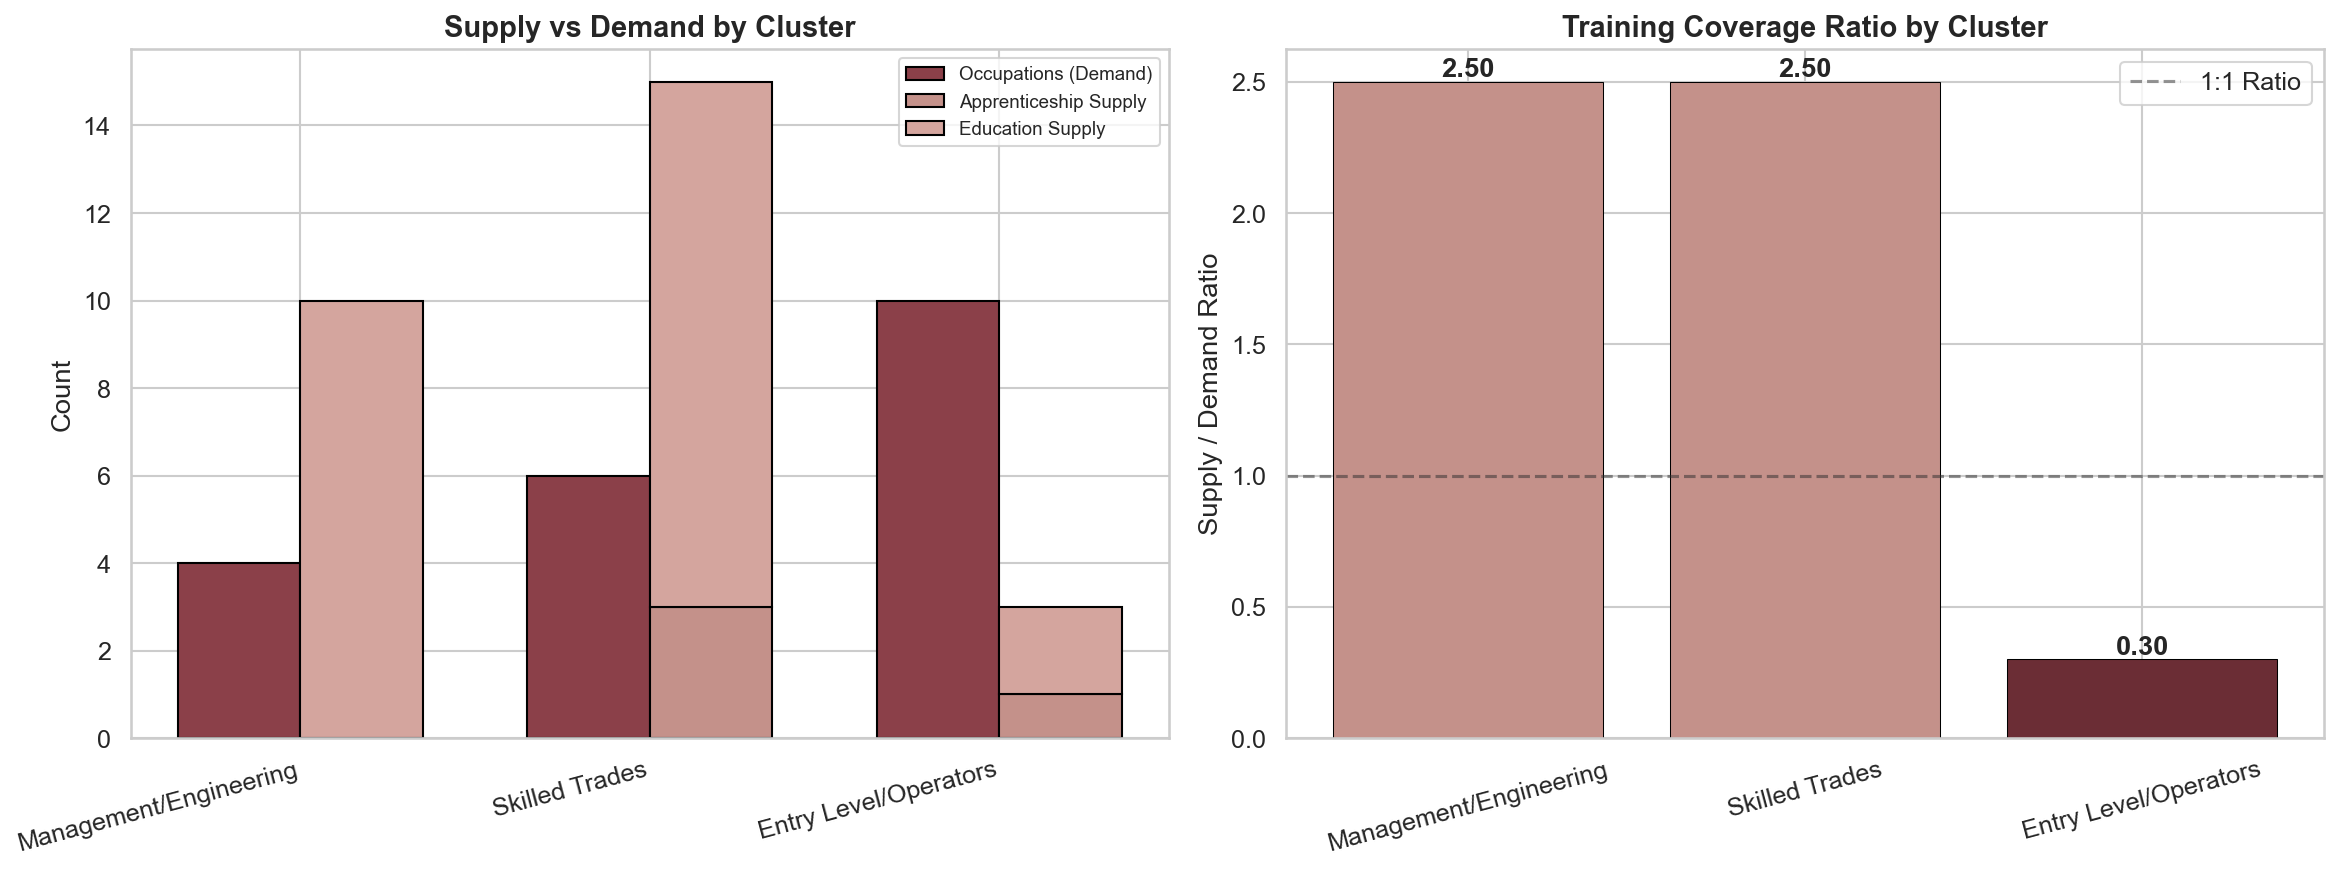
\includegraphics[width=0.88\linewidth]{supply_demand_gap.png}
\caption{Supply-demand gap by cluster. Dark bars (right panel) indicate
clusters where Coverage Ratio $< 1.0$. Entry Level/Operators
has the most severe training shortfall.}
\label{fig:gap}
\end{figure}

\begin{figure}[H]
\centering
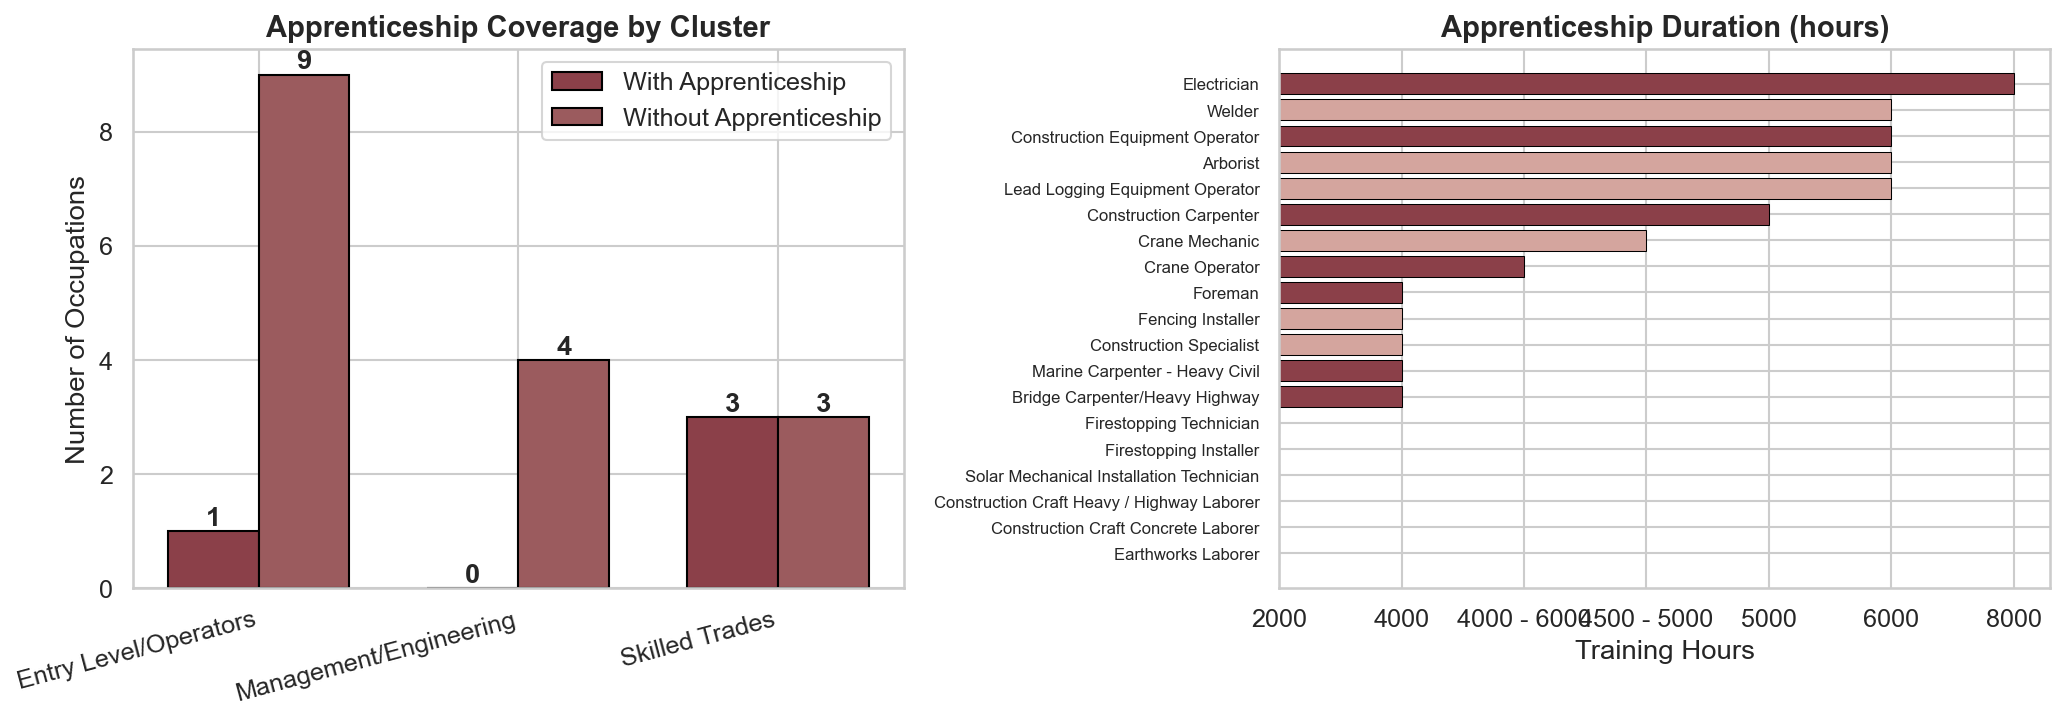
\includegraphics[width=0.88\linewidth]{apprenticeship_coverage.png}
\caption{Apprenticeship pathway coverage by cluster and
occupation. Only 7 of 19 apprenticeships map to the 20
occupations in scope.}
\label{fig:app_coverage}
\end{figure}

\begin{figure}[H]
\centering
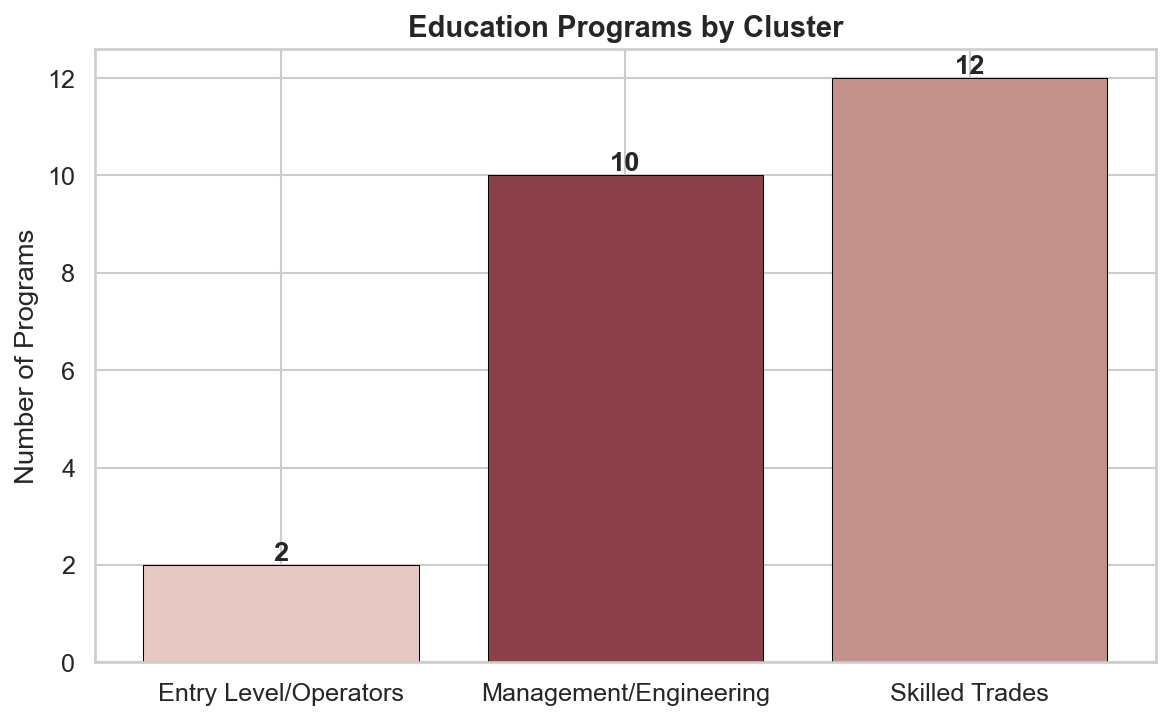
\includegraphics[width=0.88\linewidth]{education_coverage.png}
\caption{Education program coverage by cluster after mapping
correction (CC: 12/14 matched; UMaine: 8/10 matched).}
\label{fig:edu_coverage}
\end{figure}

\subsection{Track A: Skills-Based Clustering}

\paragraph{Preprocessing.}
The 120-dimensional feature matrix was standardized using
\texttt{StandardScaler} to ensure equal weighting across
features with different natural scales.

\paragraph{Dimensionality reduction.}
PCA was applied to the scaled matrix. The first principal
component (\textbf{PC1: Cognitive \& Communication Complexity})
explains 53.6\% of total variance, capturing oral expression,
reading comprehension, time management, and mathematical
reasoning --- skills that distinguish higher-complexity,
knowledge-intensive occupations from operational roles.
The second component (\textbf{PC2: Perceptual \& Sensory
Coordination}) explains 9.0\% of variance and is dominated by
visual color discrimination, near vision, time-sharing, and
auditory attention --- abilities that characterize hands-on
operational roles. Together, PC1 and PC2 capture 62.7\% of
total variance and reflect high inherent structure in the
occupation feature space.

\paragraph{Clustering.}
K-Means clustering was applied with $k=3$, selected via elbow
method and silhouette analysis. The resulting silhouette score
of 0.315 indicates moderate but meaningful cluster separation,
appropriate given the small sample ($n=20$) and high-dimensional
input. DBSCAN was evaluated as an alternative but proved
unsuitable due to the uniform density structure of the feature
space at this scale.

\begin{figure}[H]
\centering
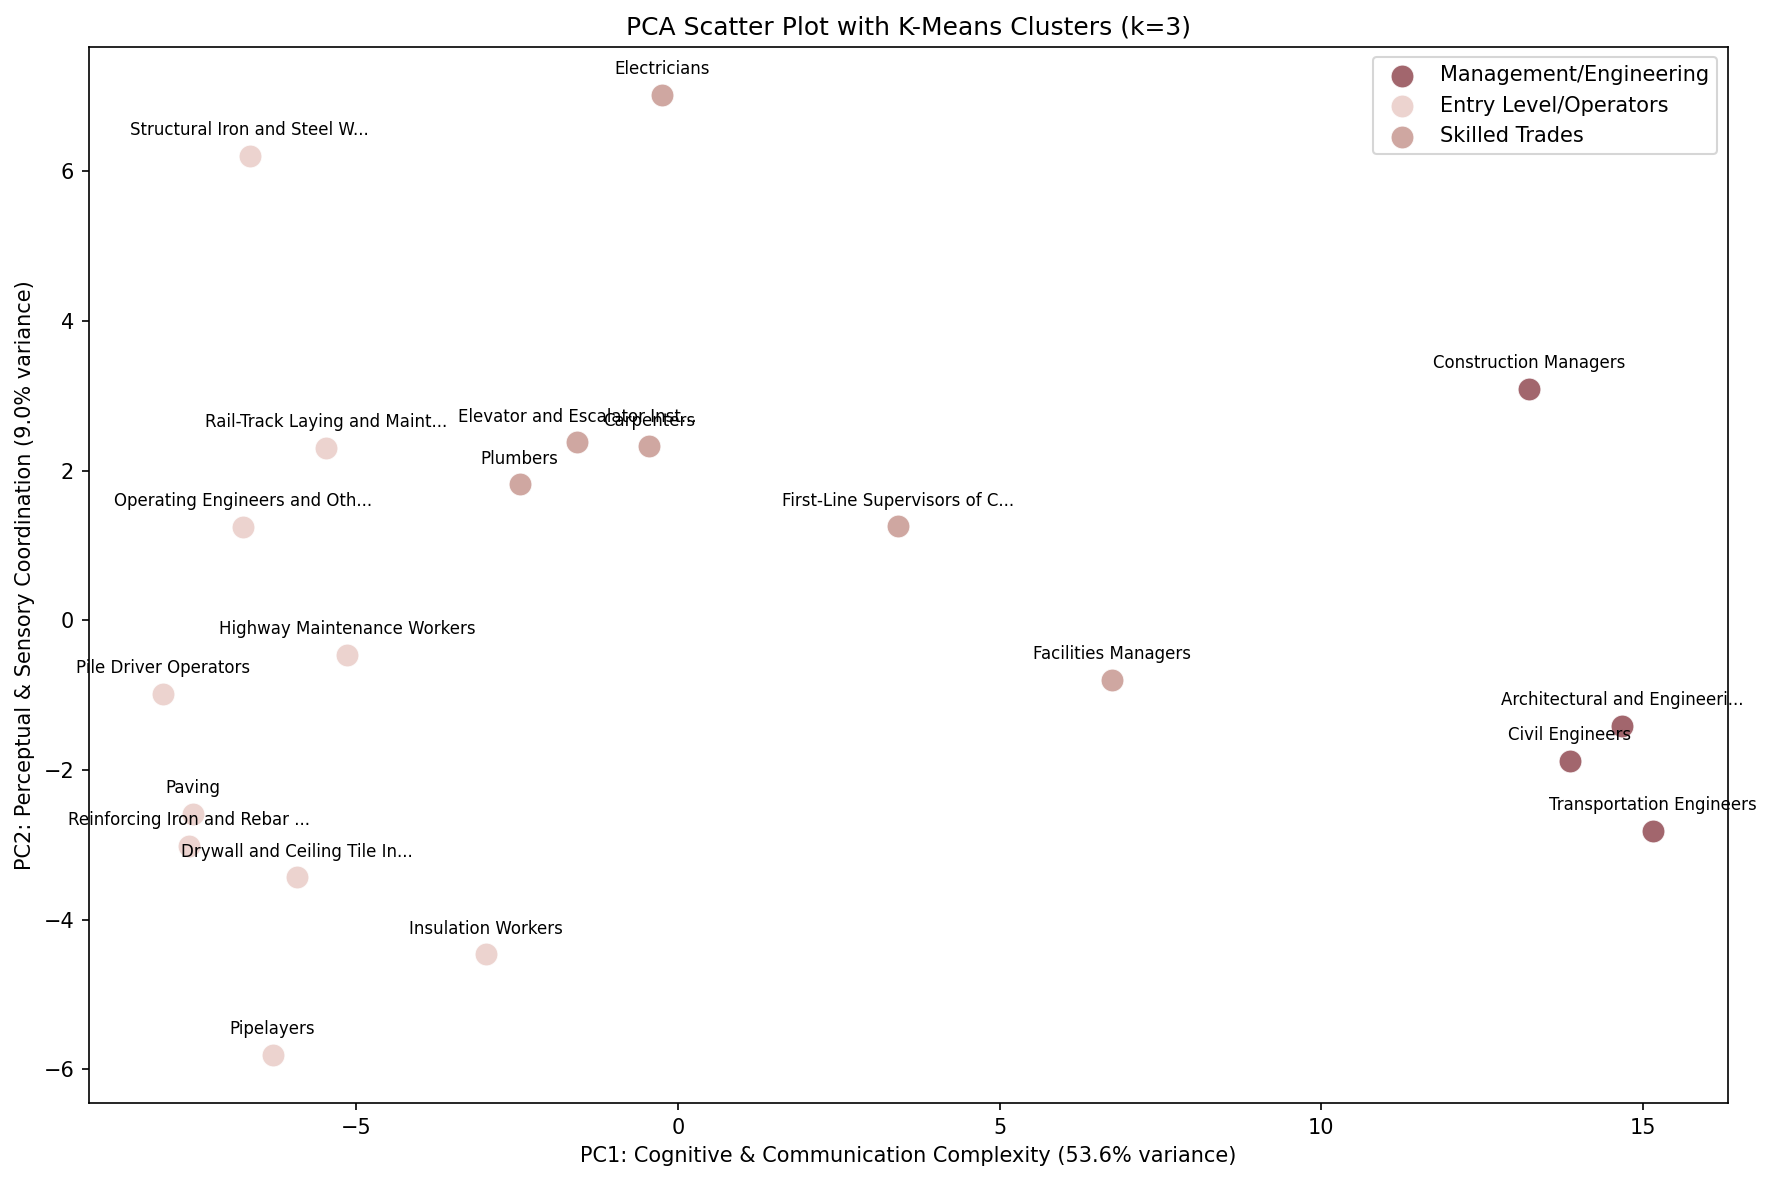
\includegraphics[width=0.88\linewidth]{pca_scatter.png}
\caption{PCA scatter plot with K-Means cluster assignments
($k=3$). The horizontal axis (PC1: Cognitive \& Communication
Complexity, 53.6\%) separates Management/Engineering from
Entry Level clusters. The vertical axis (PC2: Perceptual \&
Sensory Coordination, 9.0\%) distinguishes operational and
hands-on roles from knowledge-intensive ones.}
\label{fig:pca}
\end{figure}

The three clusters shown in Figure~\ref{fig:pca} correspond to
meaningful occupational groupings summarized in
Table~\ref{tab:clusters}. Alignment with O*NET Job Zones
provides external validation: Management/Engineering occupations
require bachelor's degrees or higher (Zones 4--5), while Entry
Level/Operators require only short-term training (Zone 2).

\begin{table}[H]
\centering
\caption{Cluster Composition and Job Zone Alignment}
\label{tab:clusters}
\begin{tabular}{lcc}
\toprule
\textbf{Cluster} & \textbf{Occupations} & \textbf{Job Zones} \\
\midrule
Management / Engineering & 4  & 4--5 \\
Skilled Trades           & 6  & 2--3 \\
Entry Level / Operators  & 10 & 2    \\
\midrule
\multicolumn{3}{l}{\small Overall silhouette score: 0.315} \\
\bottomrule
\end{tabular}
\end{table}

Figure~\ref{fig:heatmap} shows the top distinguishing features
for each cluster. Management/Engineering occupations score
highest on knowledge of Engineering and Technology, while Entry
Level/Operators are characterized by equipment operation and
monitoring skills.

\begin{figure}[H]
\centering
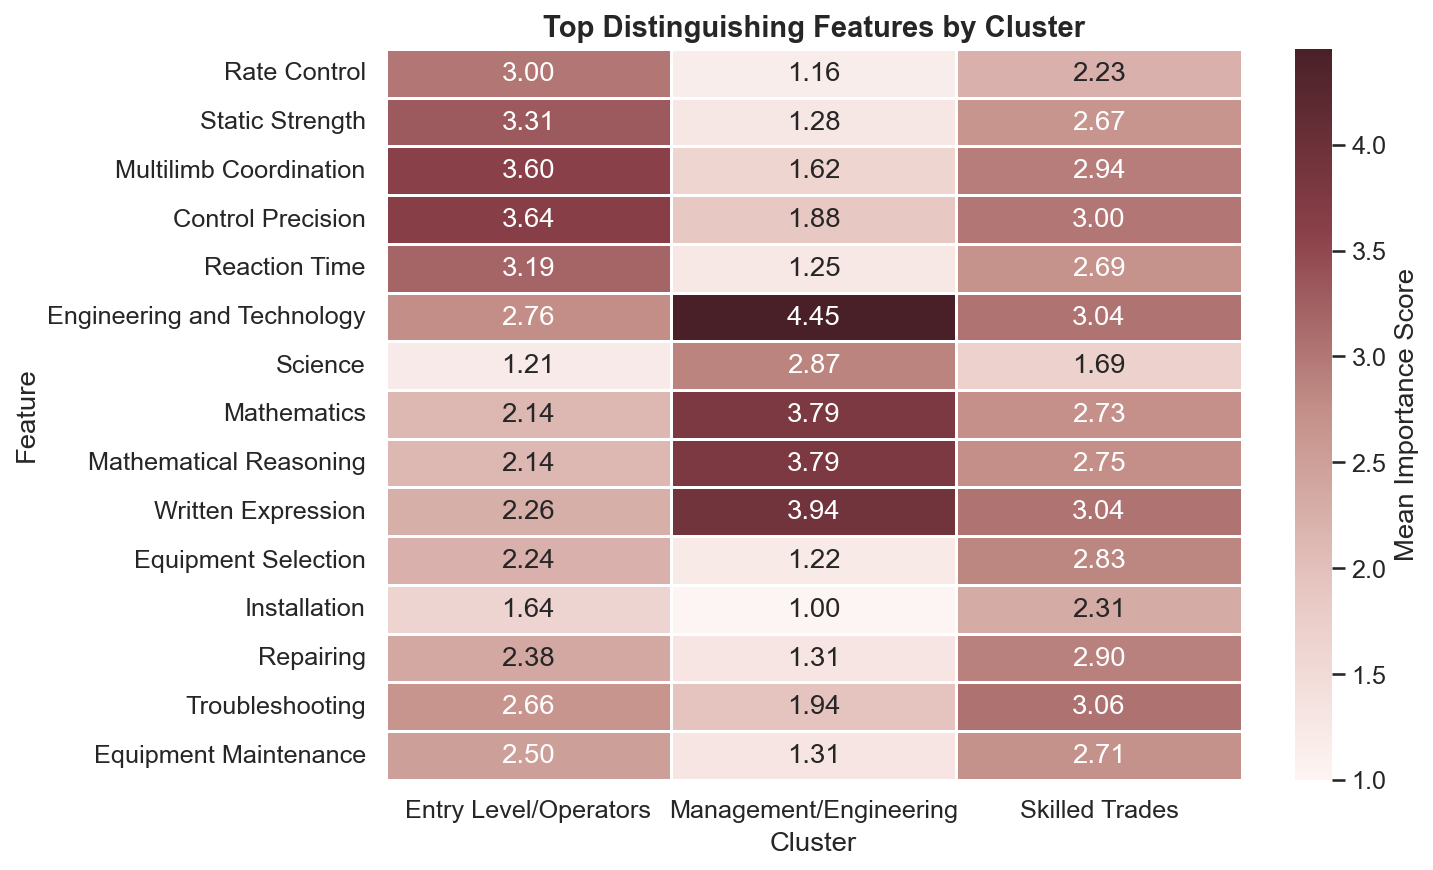
\includegraphics[width=0.88\linewidth]{skill_profiles_heatmap.png}
\caption{Heatmap of top distinguishing O*NET features by
cluster. Values represent mean importance scores (scale 1--5).}
\label{fig:heatmap}
\end{figure}

\subsection{Track B: Text Clustering and Topic Modeling}

\paragraph{Text collection.}
Occupation descriptions were enriched using the O*NET API v2,
combining tasks, work activities, and technology fields into a
single text document per occupation (average 1,417 characters).

\paragraph{Vectorization.}
TF-IDF vectorization \cite{salton1988} with 200 features, unigram and bigram
tokens, and \texttt{min\_df=2} was applied to the 20-document
corpus.

\paragraph{K-Means on text features.}
K-Means clustering on TF-IDF vectors yielded a silhouette score
of 0.103 --- lower than Track A but expected given that 20
documents is a very small corpus for text-based clustering.

\paragraph{NMF topic modeling.}
Non-negative Matrix Factorization (NMF) with 3 components
extracted three interpretable topics, shown in
Table~\ref{tab:topics} and visualized in
Figure~\ref{fig:nmf}.

\begin{table}[H]
\centering
\caption{NMF Topics Extracted from O*NET Occupation Text}
\label{tab:topics}
\begin{tabular}{lll}
\toprule
\textbf{Topic} & \textbf{Label} & \textbf{Top Keywords} \\
\midrule
0 & Equipment Operations        & equipment, machine, operate, software \\
1 & Engineering \& Management   & construction, design, project, engineering \\
2 & Installation \& Fabrication & steel, install, blueprints, pipe \\
\bottomrule
\end{tabular}
\end{table}

\begin{figure}[H]
\centering
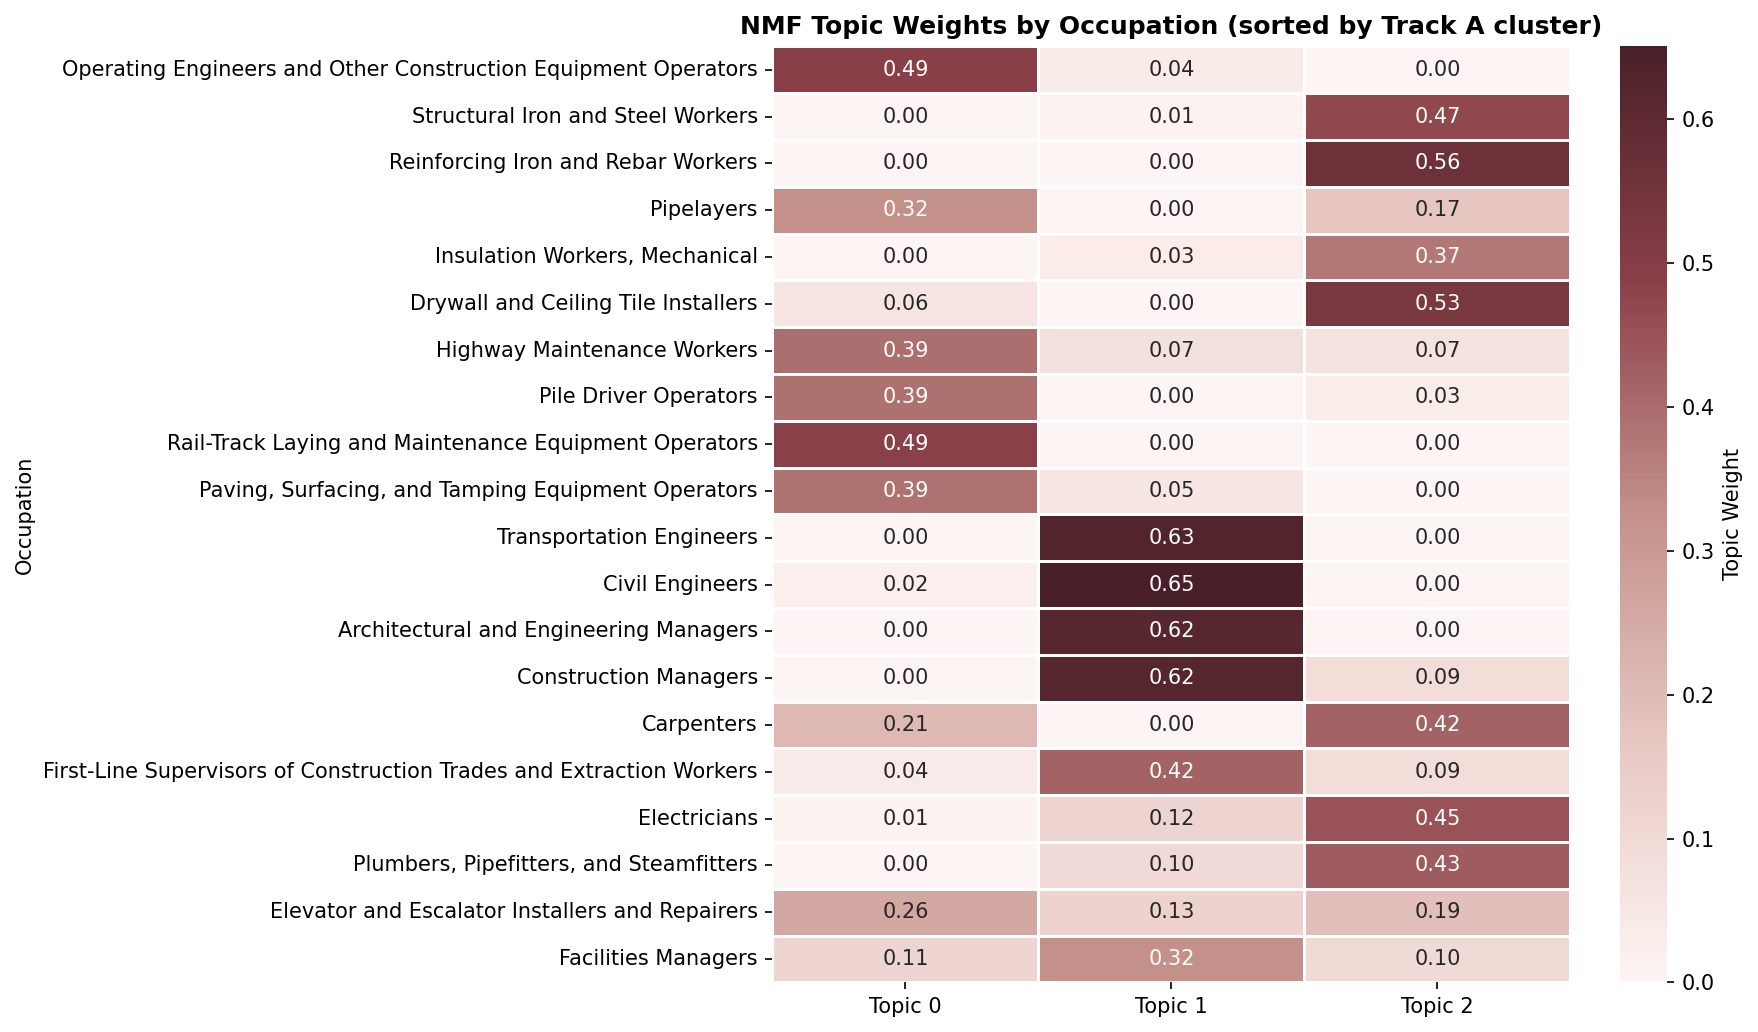
\includegraphics[width=0.88\linewidth]{topic_modeling_results.png}
\caption{NMF topic weight heatmap by occupation, sorted by
Track A cluster assignment. Management/Engineering occupations
load strongly on Topic 1; Entry Level/Operators on Topic 0.}
\label{fig:nmf}
\end{figure}

Cross-validation with Track A shows that the
Management/Engineering cluster achieves 4/4 perfect topic
alignment. Overall agreement between NMF topic assignment and
K-Means cluster is 65\% (Adjusted Rand Index = 0.269),
reflecting meaningful but imperfect correspondence --- as
expected when comparing skill-profile clustering with
text-derived topics.

\subsection{Network Analysis}

\paragraph{Graph construction.}
A career path network was constructed with 20 occupation nodes.
Edges were drawn from two sources: (1) O*NET Related Occupations
relationships (51 edges, representing officially recognized
career pathways), and (2) cosine similarity edges where
pairwise similarity of scaled feature vectors exceeded 0.95.
The resulting graph has density = 0.268 and forms a single
connected component.

\paragraph{Centrality metrics.}
Three centrality measures were computed to identify structurally
important occupations, summarized in Table~\ref{tab:centrality}.

\begin{table}[H]
\centering
\caption{Top Occupations by Network Centrality Metric}
\label{tab:centrality}
\begin{tabular}{lll}
\toprule
\textbf{Metric} & \textbf{Occupation} & \textbf{Value} \\
\midrule
Degree (hub)        & Structural Iron \& Steel Workers & 10    \\
Betweenness (bridge)& Electricians                     & 0.244 \\
PageRank            & Structural Iron \& Steel Workers & 0.092 \\
\bottomrule
\end{tabular}
\end{table}

Structural Iron \& Steel Workers functions as a network hub ---
connected to the most other occupations --- suggesting it is a
pivotal role within the Maine construction ecosystem.
Electricians, despite lower degree, have the highest betweenness
centrality, indicating they serve as a critical bridge between
clusters and represent a key skill transfer pathway.

\paragraph{Community detection.}
Louvain community detection \cite{blondel2008} identified 3 communities
(ARI = 0.279 vs.\ K-Means clusters), with 100\% agreement on
the Management/Engineering grouping. The moderate overall ARI
reflects that network topology and skill-profile similarity
capture related but distinct aspects of occupational structure.

% ─────────────────────────────────────────────────────────────
\section{Results}

\subsection{Occupational Clustering}

All three analytical methods independently identify the same
three-group structure among the 20 Maine construction
occupations, as summarized in Table~\ref{tab:convergence}.

\begin{table}[H]
\centering
\caption{Cross-Method Convergence on Three-Group Structure}
\label{tab:convergence}
\begin{tabular}{llll}
\toprule
\textbf{Method} & \textbf{Groups} & \textbf{Mgmt/Eng Match} & \textbf{ARI vs.\ K-Means} \\
\midrule
K-Means (Track A)   & 3 & Reference   & ---   \\
NMF Topics (Track B)& 3 & 4/4 (100\%) & 0.269 \\
Louvain (Network)   & 3 & 4/4 (100\%) & 0.279 \\
\bottomrule
\end{tabular}
\end{table}

The convergence is notable: three methods operating on fundamentally
different representations --- numeric skill profiles, unstructured
occupation text, and a relational career path graph --- all recover
the same Management/Engineering, Skilled Trades, and Entry
Level/Operators partition. The Management/Engineering cluster achieves
100\% agreement across all three methods, providing the strongest
structural signal. The moderate ARI values (0.269--0.279) for the
remaining two clusters are expected: NMF and Louvain capture
textual and topological similarity respectively, which partially
diverge from pure skill-profile distance at the Skilled Trades
and Entry Level boundary.

External validation against O*NET Job Zones confirms the
clustering is meaningful: Management/Engineering occupations
(Job Zones 4--5) require at least a bachelor's degree, while
Entry Level/Operators (Job Zone 2) require only short-term
on-the-job training. The K-Means silhouette score of 0.315
indicates moderate separation, appropriate for a dataset of
only 20 occupations.

\subsection{Network Structure}

Within the career path network, Structural Iron \& Steel Workers
(degree = 10, PageRank = 0.092) is the most connected occupation
and functions as the ecosystem hub. Electricians, despite having
lower degree, hold the highest betweenness centrality (0.244),
indicating they serve as the primary bridge between the Skilled
Trades and Management/Engineering clusters. This suggests
Electricians represent a high-leverage upward mobility pathway
in the Maine construction workforce.

\subsection{Supply-Demand Gap}

The supply-demand gap analysis reveals a clear training shortfall
concentrated in the Entry Level/Operators cluster. With 10
occupations but only 1 mapped apprenticeship pathway, this
cluster has the lowest coverage ratio of the three. By contrast,
Skilled Trades benefits from 12 of 14 community college programs
correctly mapped after data correction, and Management/Engineering
is relatively well served by UMaine engineering degree programs
(8 of 10 matched). Table~\ref{tab:gap} summarizes coverage by
cluster.

\begin{table}[H]
\centering
\caption{Training Coverage by Cluster}
\label{tab:gap}
\begin{tabular}{lccc}
\toprule
\textbf{Cluster} & \textbf{Occupations} & \textbf{Apprenticeships} & \textbf{CC / UMaine Programs} \\
\midrule
Management / Engineering & 4  & 2 & 8 UMaine \\
Skilled Trades           & 6  & 4 & 12 CC    \\
Entry Level / Operators  & 10 & 1 & 0 CC / UMaine \\
\bottomrule
\end{tabular}
\end{table}

\subsection{Recommendation Prototype}

The \textit{CareerDrive} Streamlit application operationalizes
the clustering and network results into three user-facing pages.
The Career Match page accepts a job seeker's plain-language
background description across seven skill categories and returns
ranked occupation matches via cosine similarity, together with
cluster membership and available training pathways. This
constitutes a working prototype of the Level 2 product envisioned
in the client roadmap.

% ─────────────────────────────────────────────────────────────
\section{Discussion}

\subsection{What the Results Mean}

The convergence of three independent methods on the same
three-cluster structure provides confidence that these groupings
reflect genuine occupational differences rather than artifacts
of any single algorithm or data representation. The alignment
with O*NET Job Zones further supports external validity.

The supply-demand gap finding has direct policy implications:
resources for apprenticeship and training program development
should prioritize the Entry Level/Operators cluster, which
includes roles such as Pipelayers, Drywall Installers, and
Highway Maintenance Workers --- occupations with low barriers to
entry but insufficient structured training pathways in Maine.

\subsection{How Results Can Be Used}

The \textit{CareerDrive} Streamlit prototype demonstrates three
concrete use cases for MaineDOT:

\begin{enumerate}
    \item \textbf{Industry Dashboard}: Gives MaineDOT staff a
    view of the company ecosystem and training coverage gaps by
    cluster.
    \item \textbf{Career Path Map}: An interactive force-directed
    network visualization showing how occupations relate by skill
    similarity and official O*NET pathways, supporting workforce
    planning discussions.
    \item \textbf{Career Match}: Allows job seekers to describe
    their background in plain language and receive occupation
    recommendations with training pathway information --- a
    prototype of the Level 2 product envisioned by the client.
\end{enumerate}

% ─────────────────────────────────────────────────────────────
\section{Limitations}

\begin{enumerate}
    \item \textbf{Small sample size.} With only 20 occupations,
    clustering results are sensitive to random seed
    initialization. The silhouette score of 0.315 indicates
    moderate separation; conclusions should be interpreted
    with caution and validated as the occupation scope expands.

    \item \textbf{Supply-side metric is approximate.} Coverage
    Ratio treats all programs equally regardless of enrollment
    capacity. A 5-person certificate program and a 200-seat AAS
    degree count equally in our current analysis.

    \item \textbf{Data quality required manual correction.} The
    CC program data in the client Excel mixed course rows with
    non-course content (funding initiatives, lab descriptions).
    After filtering to known college codes, valid records
    decreased from 21 to 14. Mapping corrections increased
    matched programs from 5/21 to 12/14.

    \item \textbf{Apprenticeship scope limitation.} 7 of 19
    apprenticeship programs map to our 20 defined occupations.
    The remaining 12 target roles (e.g., Welders, Plumbers) fall
    outside our defined occupation scope --- this is a research
    scope decision, not a data gap.

    \item \textbf{Static data.} All company and program records
    reflect a single point in time. The prototype does not
    integrate live job listings or real-time enrollment data.
\end{enumerate}

% ─────────────────────────────────────────────────────────────
\section{Future Work}

Based on the client's three-phase roadmap and our findings, we
recommend the following next steps:

\begin{enumerate}
    \item \textbf{Level 2 full build.} Integrate real-time job
    listing APIs (Indeed, LinkedIn) and live program enrollment
    data to replace the current static snapshot.

    \item \textbf{Level 3: conversational AI career coach.} The
    client roadmap envisions a small language model (SLM) trained
    on DOT-specific data. Our occupation clusters and career path
    network could serve as structured knowledge for
    retrieval-augmented generation (RAG).

    \item \textbf{Expand occupational scope.} Extend from 20
    construction occupations to the full Maine transportation
    infrastructure sector, including aviation, maritime, and
    urban planning roles.

    \item \textbf{Geographic dimension.} Incorporate county-level
    employment and wage data from BLS to enable regional
    supply-demand analysis within Maine.

    \item \textbf{Feedback loop.} Log Career Match usage patterns
    to refine the recommendation model over time, moving from
    cosine similarity toward a learned ranking model.
\end{enumerate}

% ─────────────────────────────────────────────────────────────
\begin{thebibliography}{9}

\bibitem{onet}
National Center for O*NET Development.
\textit{O*NET 30.2 Database}.
U.S.\ Department of Labor, Employment and Training
Administration, 2024.
\url{https://www.onetcenter.org/database.html}

\bibitem{nedelkoska2018}
Nedelkoska, L., \& Quintini, G. (2018).
Automation, skills use and training.
\textit{OECD Social, Employment and Migration Working Papers},
No.\ 202.
\url{https://doi.org/10.1787/2e2f4eea-en}

\bibitem{decorte2021}
Decorte, P., Poot, J., \& Smeets, M. (2021).
Jobbert: Understanding job titles through skills.
\textit{arXiv preprint} arXiv:2109.09605.

\bibitem{alabdulkareem2018}
Alabdulkareem, A., Frank, M.\ R., Sun, L., et al.\ (2018).
Unpacking the polarization of workplace skills.
\textit{Science Advances}, 4(7), eaao6030.
\url{https://doi.org/10.1126/sciadv.aao6030}

\bibitem{blondel2008}
Blondel, V.\ D., Guillaume, J.-L., Lambiotte, R., \&
Lefebvre, E. (2008).
Fast unfolding of communities in large networks.
\textit{Journal of Statistical Mechanics: Theory and Experiment},
2008(10), P10008.
\url{https://doi.org/10.1088/1742-5468/2008/10/P10008}

\bibitem{salton1988}
Salton, G., \& Buckley, C. (1988).
Term-weighting approaches in automatic text retrieval.
\textit{Information Processing \& Management}, 24(5), 513--523.
\url{https://doi.org/10.1016/0306-4573(88)90021-0}

\end{thebibliography}

\end{document}